% This is samplepaper.tex, a sample chapter demonstrating the
% LLNCS macro package for Springer Computer Science proceedings;
% Version 2.20 of 2017/10/04
%
\documentclass[runningheads]{llncs}
%
\usepackage{amsmath}
\usepackage{amssymb}
\usepackage{booktabs} % For pretty tables
\usepackage{caption} % For caption spacing
\usepackage{subcaption}
\usepackage{graphicx}
\usepackage{pgfplots}
\usepackage[all]{nowidow}
\usepackage[utf8]{inputenc}
\usepackage{tikz}
\usetikzlibrary{er,positioning,bayesnet}
\usepackage{multicol}
\usepackage{algpseudocode,algorithm,algorithmicx}
\usepackage{hyperref}
\usepackage[inline]{enumitem} % Horizontal lists
\newcommand{\indentitem}{\setlength\itemindent{20pt}}

\graphicspath{{latex/}}
\newcommand{\card}[1]{\left\vert{#1}\right\vert}
\newcommand*\Let[2]{\State #1 $\gets$ #2}
\newcommand\qfrac[3][1pt]{\frac{%
		\ThisStyle{\addstackgap[#1]{\SavedStyle#2}}}{%
		\ThisStyle{\addstackgap[#1]{\SavedStyle#3}}%
}}


\newcommand{\F}{\ensuremath{\mathbb{F}}}
\newcommand{\B}{\ensuremath{\mathbb{B}}}
\newcommand{\LL}{\ensuremath{\mathbb{L}}}
\newcommand{\Me}{\ensuremath{\mathbb{M}_e^{\text{eff}}}}
\newcommand{\D}{\ensuremath{\text{D}}}
\renewcommand{\d}{\ensuremath{\text{d}}}
\pgfplotsset{compat=1.14}

\renewcommand{\topfraction}{0.85}
\renewcommand{\bottomfraction}{0.85}
\renewcommand{\textfraction}{0.15}
\renewcommand{\floatpagefraction}{0.8}
\renewcommand{\textfraction}{0.1}
\setlength{\floatsep}{3pt plus 1pt minus 1pt}
\setlength{\textfloatsep}{3pt plus 1pt minus 1pt}
\setlength{\intextsep}{3pt plus 1pt minus 1pt}
\setlength{\abovecaptionskip}{2pt plus 1pt minus 1pt}


\begin{document}
%
\title{A thermodynamically consistent poro-visco-elastic model of Extracellular Matrix}
%
\titlerunning{Mechanical Properties of ECM}
% If the paper title is too long for the running head, you can set
% an abbreviated paper title here
%
\author{Giulia Laura Celora}
%
%\authorrunning{F. Author et al.}
% First names are abbreviated in the running head.
% If there are more than two authors, 'et al.' is used.
%
\institute{Mathematical Institute, University of Oxford}
%
\maketitle              % typeset the header of the contribution
%
\begin{abstract}

\end{abstract}
%
%
%
\section{Introduction}

In tissues, cells are mainly surrounded by extracellular matrix (ECM), a soft porous media mixed with interstitial fluid and made up of networks of polymer chains and charged proteins. \textit{In vitro} studies have shown that ECM rigidity and shear stresses due to the flow of interstitial fluid can promote malignant phenotypes in a population of initially normal cells, impact on cell proliferation and differentiation \cite{ex3}. Further experiments have shown that tumour development is often associated with a stiffening of the tissue compared to the surrounding healthy one \cite{ex4}. This causes cells to be exposed to higher compressive stresses and the blood vessels to collapse, thus impeding the diffusion of substances in the extra-cellular environment. Hence, numerous therapies are less effective \cite{ecm2}. Based on such evidence, it is now widely accepted that, unlike originally thought, biological process are not simply regulated by biochemical signals but by the complex interplay of mechanical and chemical stimuli.
 
Given the different physical nature and scale of phenomena involved, coupling micro-environment and cell behaviours is a problem of high complexity. This requires understanding processes occurring at different temporal and spatial scales and how they interplay to determine the macroscopic behaviour of a tissue, whether healthy or damaged. Despite experiments probing the micro-scale are nowadays possible, these are usually limited to controlled environment in contrast to \textit{in vivo} conditions. On the other hand, we can easily measure macroscopic properties of tissue. Hence, we need quantitative models able to link this tissue to cellular scale, so to extrapolate from the data information the environment cell perceive. In order for this to be possible, alongside experiments, it is necessary to develop a theoretical framework able to capture both the biology and physics involved and which is consistent with the known universal laws of Nature \cite{NET}. Having such knowledge on the cell micro-environment can lead to the development of novel therapies and completely change our approach to drug design.  

As it will be discussed in Section \ref{ECMcomp}, the ECM can be classified as polyelectrolyte gel \cite{ecm1,ecm2}, i.e. hydrogels with charged group. Besides being largely present in the natural world, synthetic polyelectrolytes are currently employed for a wide range of applications, such as drug delivery, biomedical devices, scaffolds for tissue engineering and soft robotics \cite{hydroex3,hydroex2,hydroex1,hydroex4}. Hence, there has been a growing interest in the soft matter community in understanding their behaviour and translating it into mathematical models. In particular, research has been focusing on the phenomena of swelling, i.e. large deformation due to absorption of water, and the diffusion transport and release of solution \cite{DROZDOV+,DROZDOVph,Reviewpolyel,swell2}.

With the development of new experimental techniques such as Atomic Force Microscopy (AFM), the local mechanical properties of a material can be measured with nanometre precision \cite{viscoporo}. When tested at this scale, soft tissues, as well as hydrogels, have been found to be visco-elastic \cite{ex5}. As their solid skeleton, i.e. polymer network, is deformed, it can change its conformation to a most entropically favourable one thus dissipating energy. Where purely elastic solids deformed instantaneously, viscoelastic materials instead have time-dependent deformation due to the irreversible nature of the process. 
Despite these experimental evidences, theoretical studies on visco-elastic soft materials remain limited. Most of the literature has been proposing poro-elastic models, which account for the dissipation of energy due to the transport of solutions but neglect the visco-elastic response of the material itself \cite{Article1}. While this assumption might be valid for certain applications, the empirical studies previously mentioned highlight the need of including this component in the study of living tissues. 

Our works aims to develop a continuum mathematical model of the extracellular matrix which is consistent with the laws of thermodynamics, which accounts for its poro-visco-elastic properties and the coupling of mechanical, transport and electrical phenomena. Nonetheless, our results are more widely applicable to the study of polyelectrolyte gels. At our present knowledge, there is no previous work in the literature capturing all these aspects in a thermodynamic consistent model. In \cite{ecm1,ecm2} Xue et al.~ develop a nonlinear poroelastic theory for ECM, which couples all three physical phenomena but does not include viscous dissipation. In \cite{Jeru}, the authors couple mechano-electrophysiological effects including the viscous dissipation but neglect transport; Caccavo et al.~ \cite{Article1} propose a poro-viscoelastic model for neutral hydrogel, thus excluding electrical effects. Following these previous work, we will derive our model in the framework of linear non-equilibrium thermodynamics \cite{NET} accounting for multiple phases.

As discussed in \cite{viscoporo}, there are spatial and time scales which allow to decouple visco-elasticity and poro-elasticity. On one hand, nanoscale rheological testing with AFM give us information on the visco-elastic properties of the sample. For sufficiently small beads, the length scale considered in the experiment is so short that poroelastic relaxation is almost instantaneous and thus negligible. Different 1D rheological model are usually applied to fit experimental measurement: the most common for tissues and hydrogels is the \textit{Standard Linear Solid} model, see Figure \ref{SLS}, to fit the experimental data \cite{Article1,viscoporo}. The poro-elastic behaviour can instead be characterized by standard creep-relaxation test on whole sample. In this case, Darcy's law is usually applied to estimate the hydraulic conductivity and thus characterise the transport of fluid in the material \cite{Netti,viscoporo}. Despite having a good understanding of the two phenomena independently, there has been little attention to investigating how the two couples. Following a typical approach in the framework of large deformation, we will be using a multiplicative decomposition of the deformation gradient to account for the two phenomena simultaneously. 

\begin{figure}
	\begin{subfigure}{0.45\textwidth}
		\centering 
		\def\svgwidth{1.3\linewidth}
		\input{latex/images/SLStand.pdf_tex}
		\caption{}
	\end{subfigure}
	\begin{subfigure}{0.45\textwidth}
	\centering
	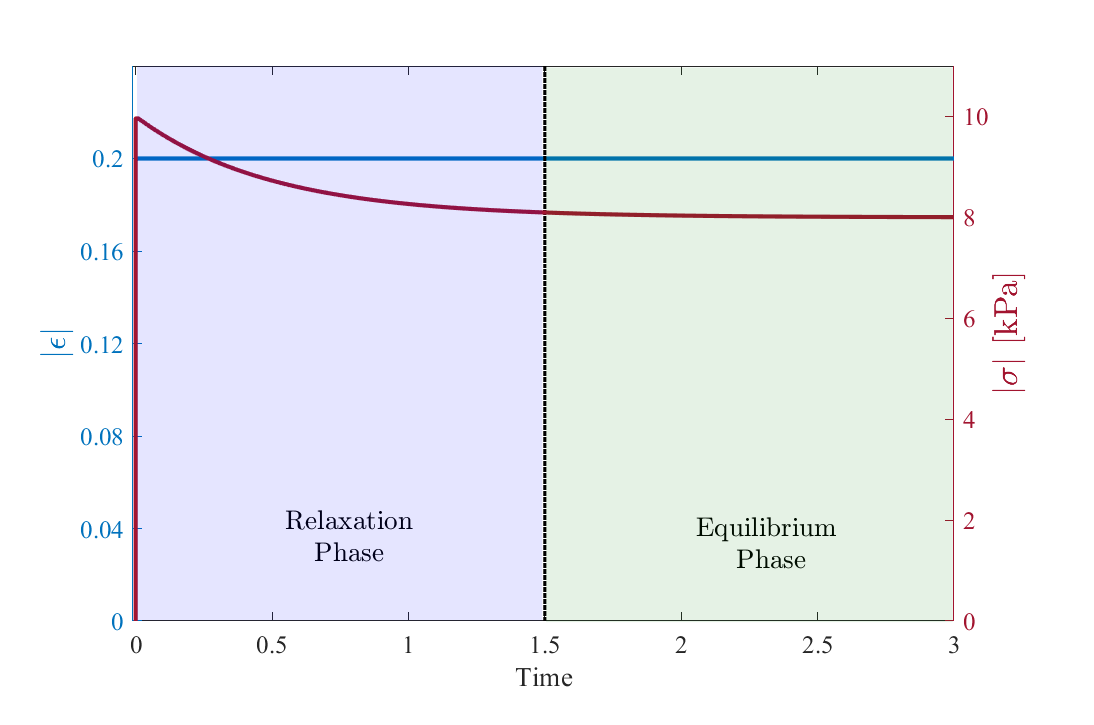
\includegraphics[scale=0.28]{images/SLS}\qquad 
	\caption{}
	\end{subfigure}

\vspace{5mm}
\begin{equation}
\begin{cases}
\sigma = E_1\epsilon+E_2\epsilon_d\\
\dot{\epsilon}_e = \dot{\epsilon} -\frac{E_2}{\eta} \epsilon_e = \dot{\epsilon} - \frac{\epsilon_e}{\tau_R}
\end{cases}
\tag{SLS}
\end{equation}
\vspace{3mm}
\caption{1D Standard Linear Solid. (a) Rheological Model; (b) Standard Response to a compression test. (1) Differential Equation for the Standard Linear Solid model in the 1D case.}
\label{SLS}
\end{figure}

In the framework of large deformation, a standard approach to the study of couple phenomena is the use of a multiplicative decomposition of the deformation gradient. We will be rely on the same idea to build our poro-visco-elatic model. In the literature of soft matter, two possible decomposition have been proposed, based on arbitrary choice, but never systematically compared. As our analysis shows, multiplicative decomposition should be treated as constitutive laws of the material and thus validated  and compared. Instead of arbitrarily choosing one of the two, we here develop both approaches, with the aim of identifying their differences and investigating experimental result which would allow us to experimentally test which one best describes the behaviour of soft tissues. 

Our work is organized as follows: in Section \ref{ECMcomp}, we discuss more in details the composition of the ECM. We then present a brief overview of Classical Irreversible Thermodynamics, which focuses on the principles later used in the derivation of our model in Section \ref{modeldev}. Common  [... FOLLOWING SECTIONS TO UPDATE AS I WRITE.]

\section{Non Equilibrium Thermodynamics.}
\label{secNET}
While equilibrium thermodynamics can describe ideal processes, it does not apply to real processes which are irreversible. In this cases, the change in the entropy of a system $\d S$ results from both the reversible exchange of energy and matter with the external environment $\d_eS$ and the internal dissipation of energy during the process $\d_iS$ \cite{NET}:
\begin{equation}
\d S = \d_eS + \d_iS, 
\end{equation}
According to the second law of thermodynamics, which applies universally to any system or any of its sub-part $\d S_i\ge 0$. It is important to notice that the second law allows transformations in which total change in entropy $d S$ of the system is negative. This occurs whenever $-\d_e S>\d_i S$ and it can lead to the spontaneous formation of complex and ordered structures such as living organisms. From this point of view, life has emerged as an efficient mechanism able to increase sufficiently the entropy of its environment \cite{JeremyEngland}.  

In this study, we will focus on isothermal processes, i.e. $T=const$. Under this assumption, as derived by Gurtin in \cite{GURTIN}, the second law of thermodynamics is equivalent to the following \textit{energy imbalance inequality}:
\begin{equation}
\frac{\d}{\d t} \left\{\int_R \psi \right\}\leq W(R) + M(R) \label{energyin}
\end{equation}
where $R$ is a arbitrary control volume of the system, $\psi$ is the Helmholtz free energy, $W(R)$ is the rate at which the environment does work on $R$ and $M(R)$ is the inflow of mass due to transport. It is important to note that, as long as the quantities involved are well defined, the energy inequality~(\ref{energyin}) holds for any isothermal process independently of the specific physical system considered. This imposes a constraint on the form of the function $\psi$ and how this depends on the other thermodynamic variables, such as temperature or pressure, which are used to describe the system. 

Non-equilibrium thermodynamics mainly focuses on defining the form of $\d_i S$, which, unlike the reversible entropy production $\d_e S$, is not a state variable but depends on the specific transformation applied to the system. 
Different theories have been proposed, \cite{NET}, each with its assumptions and specific domain of applicability. In our study we will focus on \textquotedblleft Classical Irreversible Thermodynamics'' (CIT) which was pioneered by Onsager \cite{onsager} and Prigogine \cite{prigogine} in the first half of the 20th century. One the most important assumptions of this theory is the \textit{Local Equilibrium Hypothesis}, which guarantees thermodynamic variables, including entropy, are locally well-defined, \cite{NET}. 
Consequently, we can introduce the entropy density $s=s(\mathbf{x},t)$ such that:
\begin{equation}
S = \int_{R} s \,\d V, \qquad \d s = \d_e s + \d_is, \qquad \d_is > 0, 
\end{equation}
and the local entropy production:
\begin{equation}
\sigma \equiv \frac{\d_i s}{\d t} \geq 0.
\end{equation}

Another central aspect of the theory is the introduction of \textit{thermodynamic forces} \footnote{Not to be intended in the mechanical sense} $F_m$ (causes) and \textit{thermodynamic fluxes} $J_m$ (effects) to describe the time evolution of the system during an irreversible transformation. These are related to $\sigma$ as follows:
\begin{equation}
\sigma = \sum_m F_m J_m\geq 0.
\label{2law}
\end{equation}

While the local equilibrium hypothesis is at the basis of most theories of non-equilibrium thermodynamics, the following two hypotheses uniquely identify CIT:
\begin{itemize}
	\item[1.] \textit{Linear Relation between forces $F$ and fluxes $J$}:
	\begin{equation}
	J_m = \sum_k L_{mk} F_k,\label{lin}
	\end{equation}
	where the constant $L_{mk}$ are referred to as \textbf{phenomenological coefficients};
	\item[2.] \textit{Microscopic Reversibility}: time reversibility of processes at the micro-scale. 
\end{itemize}

Starting from these two principles, in its seminal paper \cite{onsager} Onsager derives the well-known \textit{Onsager Reciprocal Relation}:
\begin{equation}
L_{mk}=L_{km}.
\end{equation}

If we now consider an isothermal transformation in the framework of CIT, alongside with the energy imbalance inequality, we have that the following must hold:

\begin{equation}
W(R)+M(R)-\frac{\d}{\d t} \left\{\int_R \psi \right\} = T \int_R \sigma \,\d V\, ,
\label{eqCIT}
\end{equation}

In the past few decades, CIT has been applied successfully to the modelling of several physical phenomena of interest for engineers, physicists and applied mathematicians. However, its validity is limited to phenomena near-equilibrium, for which a linear approximation of the flux-force relation holds. The growing interest in more complex far-from-equilibrium phenomena has pushed toward the development of a more general framework for the study of a non-equilibrium phenomena. Since this goes beyond the purpose of our study, we will not discuss it further. We just want to mention the law of steepest entropy ascent, which, according to Beretta \cite{SEA2}, seems to emerge as the fourth fundamental law of nature. In the linear regime, this principle can be used to prove Onsager's reciprocal relation \cite{SEA1}, with no reference to the microscopic reversibility hypothesis, whose validity remains instead controversial \cite{CIT}.

\section{Composition of Extracellular Matrix.}
\label{ECMcomp}
Despite the tissue-specific nature of Extracellular Matrix (ECM), as shown in Figure \ref{ECMfig} (a), this is usually composed of a network of collagen fibrils entangled with proteoglycans (PGAs) which are covalently bonded to charged chains of glycosaminoglycans (GAGs).  While collagen is mainly responsible for the mechanical behaviour of the tissue, GAGs can imbibe water, giving the extracellular matrix the ability to swell while maintaining its structural integrity. From this point of view, the ECM behaves as a polyelectrolyte gel \cite{ecm1,ecm2}. As schematically illustrated in Figure \ref{ECMfig}(b), polyelectrolyte gels are 3D networks of cross-linked polymer chains that contain ionizable functional groups. When in solution the gel swells, while the functional groups dissociate into fixed charges and mobile ions in the solution. Besides being largely present in the natural world, synthetic polyelectrolytes are currently employed for a wide range of applications, such as drug delivery, biomedical devices, scaffolds for tissue engineering and soft robotics \cite{hydroex3,hydroex2,hydroex1,hydroex4}. Given their wide industrial application, there has been a growing effort in understanding their behaviour and translating it into mathematical models. In particular, research has been focusing on the phenomena of swelling, i.e. large deformation due to absorption of water, and the diffusion transport and release of solution  \cite{DROZDOV+,DROZDOVph,Reviewpolyel,swell2}. However, only a small fraction of the study published accounts for the visco-elastic properties of the polymer network.

\begin{figure}[h]
	\begin{subfigure}{0.49\textwidth}
	\centering
	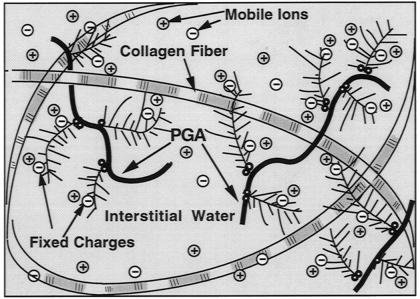
\includegraphics[scale=0.38]{images/ECM}
	\caption{}
	\end{subfigure}
	\begin{subfigure}{0.49\textwidth}
	\centering
	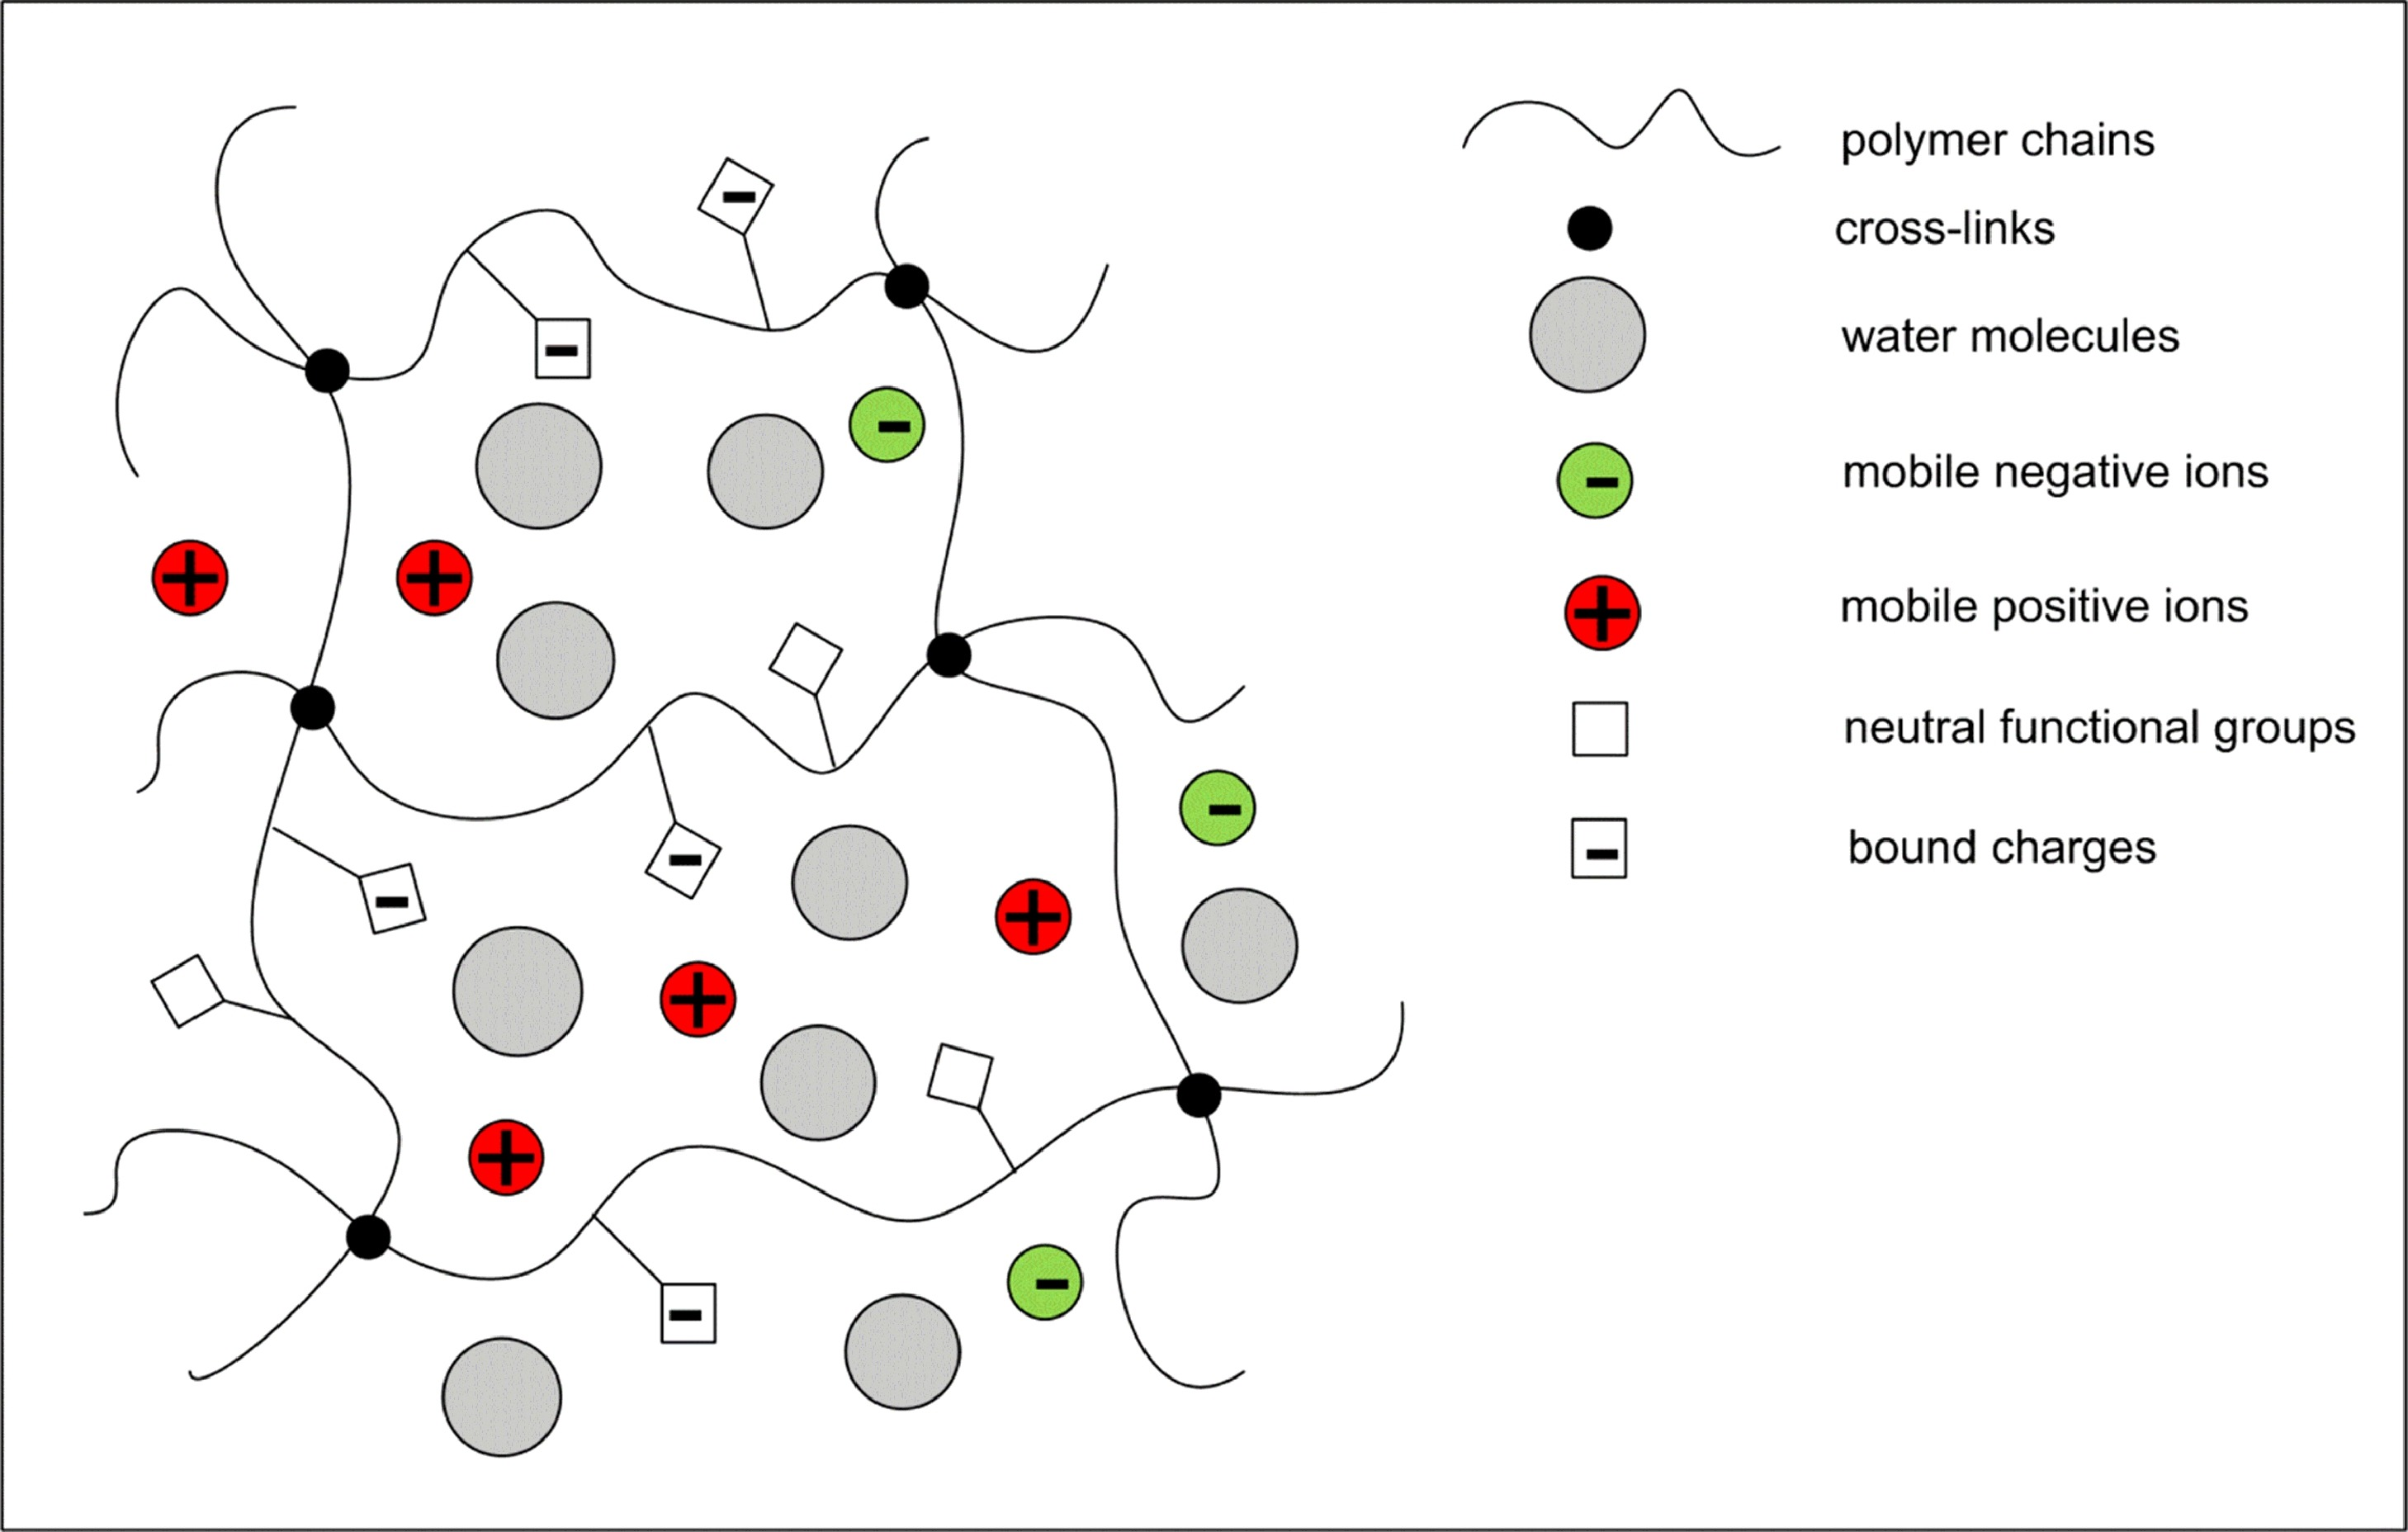
\includegraphics[scale=0.42]{images/ecmscheme.jpg}
	\caption{}
\end{subfigure}
\caption{Analogy between ECM in soft tissue and polyelectrolytes hydrogels: (a) schematic diagram of the structure of the charged hydrated articular cartilage, reproduced from \cite{pictureECM}; (b) an anionic polyelectrolyte gel modelled as a three-phase continuum, reproduced from \cite{DROZDOVph}.}
\label{ECMfig}
\end{figure}

As shown in Figure \ref{ECMfig}, the extracellular matrix falls into the definition of polyelectrolytes so that the knowledge acquired in the study of these materials can be transferred to soft tissues. For the purpose of this study, we will not explicitly distinguish between collagen, PGAs and GAGs. At the tissue level, this can be grouped into a single solid phase (the polymer networks), whose mechanical properties are treated as the average over the different components contribution. As common in multiphase models of tissue, we will assume that the matrix is isotropic and GAGs are evenly distributed on the network. While this is not a good approximation for tissue like cartilage, which are highly anisotropic, it does apply to the extracellular matrix found in other soft tissue like liver, brain and tumours. It is also important to point out that ECM has additional properties such as thermo-sensitivity and pH-sensitivity. However, both in living organisms and in experimental set-up temperature and pH are maintained fairly constant.

\section{Model Development}
\label{modeldev}
\subsection{Conservation Law.}
\label{conslaw}
As mentioned in the previous section, we here consider the ECM as a three-phase medium composed of a solid polymer network with fixed charges, a solvent (i.e. water molecules, interstitial fluid) and solutes (freely moving charges). 

We assume that the deformation of the ECM corresponds to the one of the solid network. As the tissue deform, the material element originally located at $\mathbf{X}$ in the initial configuration $\mathcal{B}_0$ is displaced to the point $\mathbf{x}$ in the current configuration $\mathcal{B}$. Such transformation is described by the deformation gradient tensor $\F= \partial \mathbf{x}/\partial \mathbf{X}$; the information about the change in ECM's volume due is encoded by $J= \det \F$. Since we assume the solid phase to be incompressible, any change in the volume can only be related to the migration of solvent and solutes molecules, whose nominal concentrations will be denoted by $C_s$ and $C_i$ respectively, $i=1,\ldots,N$ with $N$ being the number of free ion species. This lead to the molecular incompressibility condition:

\begin{equation}
 J= 1 + v_s C_s +\sum\limits_{i=1}^{N} v_i C_i
 \label{comp}
\end{equation}
where $v_m$ are the characteristic molecular volume of each species in the solution. When considering the interstitial fluid, the contribution of ions to the volume can be neglected \cite{ecm1,ecm2} so that Equation~(\ref{comp}) reduces to:

\begin{equation}
J=1+v_s C_s.
\label{inc}
\end{equation} 

Consequently, the volume fractions of fluid $\phi_f$ and solid $\phi_n$ phases in the gel are defined as:
\begin{equation}
\phi_f = \frac{v_sC_s}{1+v_sC_s}, \qquad \phi_n = \frac{1}{1+v_sC_s}.
\end{equation}
where again we are neglecting the contribution of ions to the total volume.
While $C_m$ denote the number of each molecule per unit volume in the initial configuration for the $m$-th species in the solution, the actual concentration in the current state is denoted by $c_m=C_m/J$. Throughout the derivation of the model, we will be using the index $i=1,\ldots,N$ to denote the ionic species only, while $m\in\left\{s,1,\ldots,N\right\}$ to refer to all mobile species, i.e. both the solvent and solutes.

Mass conservation must apply to all mobile species and in the initial configuration this reads:
\begin{equation}
\dot{C}_m + \nabla_0 \cdot \mathbf{J}_m = 0, \label{consmass}
\end{equation}
where $\mathbf{J}_m$ is the nominal flux per unit area in the dry state and $\nabla_0$ denote the gradient in the Lagrangian coordinates $\mathbf{X}$. Their counterparts in the actual configuration are denoted by $\mathbf{j}_m$ and $\nabla$ and are defined according to the following rules:
\begin{equation}
\mathbf{J}_m = J \F^{-1} \mathbf{j}_m, \qquad \nabla_0 (\cdot) = \F^{T} \nabla(\cdot).
\end{equation}

When considering tissues or hydrogels, inertial and gravitational effect are commonly neglected, so that the conservation of momentum for the ECM reads:

\begin{gather}
\nabla_0 \cdot \mathbb{S}=0\label{consmom},
\end{gather}

where $\mathbb{S}$ is the first Piola-Kirchoff tensor, which represents the stress state of the ECM in the initial configuration. The counterpart in the current configuration is the Cauchy stress tensor $\mathbb{T}$, which is related to $\mathbb{S}$ as follows:

\begin{equation}
\mathbb{T} = J^{-1}\mathbb{S}\F^T.
\end{equation}

The presence of free moving ions generates and electric field which is denoted by $\mathbf{E}$ and $\mathbf{e}$ in the initial and current configuration respectively. Introducing the electrostatic potential $\Phi$, we have that:
\begin{equation}
\mathbf{E}= -\nabla_0 \, \Phi, \hspace{8mm} \mathbf{e}= - \nabla \, \Phi.
\end{equation}

As in \cite{Reviewpolyel}, we consider the matrix to be a dielectric material. Consequently, the presence of the electric field generates an electric displacement $\mathbf{H}$, which must obey Gauss law of electrostatics:
\begin{equation}
\nabla_0 \cdot \mathbf{H}= Q,
\label{gauss}
\end{equation}
where $Q$ is the local total charge, which accounts for both fixed and moving charges:
\begin{equation}
Q = e\left(\sum\limits_{i} z_i C_i+z_f C_{f}\right)\, , 
\end{equation}
where $e$ is the elementary charge, $C_f$ is the concentration of fix charges and $z_m$ is the valence of the corresponding charged species. Note that $C_f$ here corresponds to the concentration of GAGs, which is assumed to be a constant a fraction of $C_s$. As for above, we can move from nominal quantities to the corresponding value in the current configuration by applying the following rules:

\begin{eqnarray}
\mathbf{H} = J \mathbf{h}\F^{-T},\\
\mathbf{E} = \F^T \mathbf{e},
\end{eqnarray}
where $\mathbf{h}$ is the electric displacement in the current configuration.

\subsection{Kinematics.}
\label{kin}

As in \cite{sarah}, we here consider that the initial state of the system $\mathcal{B}_0$ corresponds to the dry state of the gel. At any time $t$, the actual configuration of the body is $\mathcal{B}_t$. Note that in what follows we will refer to the the current configuration $\mathcal{B}_t$ as $\mathcal{B}$. 

As mentioned in the introduction, we model the ECM as a poro-visco-elastic material. As shown in Figure \ref{deformation}, there are two mechanisms that can deform the system: 
\begin{itemize}
	\item [1.] the rearrangements of molecules at the micro-scale,  which has entropic origin and result in a volume-preserving viscous deformation;
	\item[2.] the long range transport of fluid that leads to swelling, i.e. changes in the ECM's size. 
\end{itemize}

\begin{figure}[h!]
	\centering
	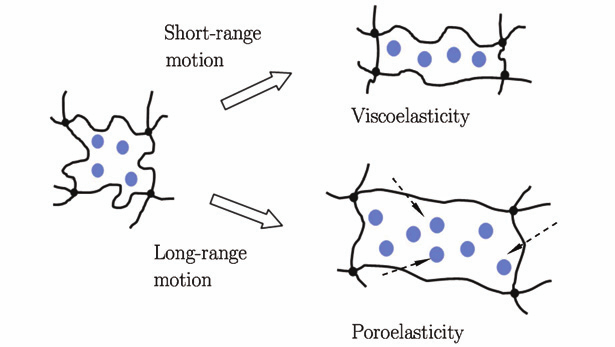
\includegraphics[scale=0.325]{images/visco_poro}
	\caption{Illustration of the molecular processes which account for the macroscopic deformation of ECM: viscosity is related to change in the conformation of the network which results in short-range movement of fluid relative to the polymers; poro-elasticity is instead responsible for the long-range diffusion of solvent molecules in the gel/tissue. Reproduced from \cite{viscoporo}.}
	\label{deformation}
\end{figure}
 
As mentioned in the introduction, we are here interested in the coupling of this two phenomena. As discussed in \cite{viscoporo}, there are spatial and time scales which allow to study the two independently. On one hand, nanoscale rheological testing with AFM give us information on the visco-elastic properties of the sample. For sufficiently small beads, the length scale considered in the experiment is so short that poroelastic relaxation is almost instantaneous and thus negligible. Different 1D rheological model are usually applied to fit experimental measurement: the most common for tissue and hydrogels is the \textit{Standard Linear Solid} model, which is illustrated in Figure \ref{figmode}(a), to fit the experimental data \cite{Article1,viscoporo}. The poro-elastic behaviour can instead be characterized by standard creep-relaxation test on whole sample. In this case, Darcy's law is usually applied to estimate the hydraulic conductivity and thus characterise the transport of fluid in the material \cite{Netti,viscoporo}. 

Despite having a good understanding of the two phenomena independently, there has been little attention to investigating how the two couple. In Figure \ref{figmode}, we have illustrated the two main approaches that have been proposed in the literature. To avoid any confusion, we will denote them as model A and model B respectively. Despite being quite similar, model B explicitly decouple the volumetric and deviatoric deformation of the system by introducing an addition spring to standard linear solid (SLS) \cite{magneto,NGUYEN,Jeru}. On the other hand, model A assumes that the model behaves as a SLS both under deviatoric and volumetric deformation.

At our knowledge, there is no systematic study in the literature that compares the two approaches and their predictions in different experiments. Instead of making an arbitrary decision, we will derive two models, one for each constitutive relation. We will then compare their predictions and investigate whether the two are consistent or can give rise to substantially different behaviour.    

As an explanatory example of the derivation of a model in the non-equilibrium thermodynamics framework, we will here fully derive the governing equation corresponding to model A. The interested reader can find the details of the derivation for model B in Appendix [Need to add the name]. 

\begin{figure}[h!]
	\centering
	\begin{subfigure}{0.32\textwidth}
		\centering
		\Large
	\def\svgwidth{0.95\linewidth}
	\input{latex/images/modelA1.pdf_tex}
	\caption{Rheological Model A}
	\label{fig1A}
	\end{subfigure}
\hspace{10mm}
	\begin{subfigure}{0.32\textwidth}
	\Large
	\def\svgwidth{0.95\linewidth}
	\input{latex/images/modelB1.pdf_tex}
	\caption{Rheological Model B}
	\label{fig1B}
\end{subfigure}

\begin{subfigure}{0.34\textwidth}
	\Large
	\def\svgwidth{1.75\linewidth}
	\input{latex/images/modelA2.pdf_tex}
	\caption{Multiplicative decomposition of Model A}
	\label{Model2}
\end{subfigure}
\vspace{5mm}
\caption{(a-b) two different rheological models for soft tissue; (c) multiplicative decomposition corresponding to model A, Equation~(\ref{dec1}).}
\label{figmode}
\end{figure}

Following a common approach in the large-deformation theory \cite{Article1,CACCAVO2,Plasto,magneto,NGUYEN,growthtum}, we base our derivation on a multiplicative decomposition of the deformation tensor $\F$, approach first proposed by Kr\"{o}ner in 1960 \cite{kro}:

\begin{equation}
\F=\F_e\F_v,\label{dec1}.
\end{equation}

As shown in Figure \ref{figmode}(a), $\F_e$ is the elastic contribution to the deformation related to the spring in branch $\mathbf{B}$. On the other hand, the term $\F_v$ accounts for the viscous flow due to the dashpot in branch $\mathbf{B}$. As illustrate in Figure \ref{figmode}(c), this multiplicative decomposition is equivalent to introducing an intermediate configuration $\mathcal{B}_v$, called natural or virtual configuration. Despite it not being a real state of the system, it can be interpreted as the state the system would be in if it was instantaneously elastically unload. 

Using Equation~(\ref{dec1}), we can compute the velocity gradient tensor $\LL$:
\begin{equation}
\LL = \dot{\F}\F^{-1} = \LL_e + \F_e \LL_v \F_e^{-1},
\end{equation}
where $\LL_e=\dot{\F}_e\F_e^{-1}$ and $\dot{\F}_v\F_v^{-1}$ are respectively the elastic and viscous velocity gradient tensor. These can be decomposed in their symmetric and skewed part:

\begin{equation}
\begin{aligned}
\LL_e = \mathbb{D}_e + \mathbb{W}_e, \ \ \mathbb{D}_e = \frac{\LL_e+\LL^T_e}{2}, \ \ \mathbb{W}_e = \frac{\LL_e-\LL^T_e}{2};\\
\LL_v = \mathbb{D}_v + \mathbb{W}_v,  \ \ \mathbb{D}_v = \frac{\LL_v+\LL^T_v}{2}, \ \ \mathbb{W}_v = \frac{\LL_v-\LL^T_v}{2}.
\end{aligned}
\end{equation}

The decomposition~(\ref{dec1}) is not unique, as stress state in $\mathcal{B}_v$ would not change under any arbitrary rigid-body rotation \cite{multdec}. As suggested by \cite{Plasto}, in the case of isotropic material, it is reasonable to assume the viscous flow to be irrotational, i.e. $\mathbb{W}_v=\mathbb{O}$, so that $\LL_v \equiv \mathbb{D}_v$.
As mentioned before, the physical nature of the viscous deformation, molecular rearrangement. This requires to introduce an additional constraint:
\begin{equation}
J_v=\det \F_v= 1.\label{Jv}
\end{equation}

Note that in the second model B, this condition is naturally imposed as the only volumetric contribution to the stress is related to $\F_{vol}$.
Despite condition~(\ref{Jv}) being common assumption in the study of hydrogels and soft tissue, there are few exceptions \cite{Article1,CACCAVO2,wang} model. Consequently, our results will differ from the one in the paper mentioned. 
 
\subsection{Energy Balance Inequality.}

As mentioned in Section \ref{secNET}, according to how the system exchanges energy and mass with the environment, the energy imbalance imposes restrictions on the free energy $\psi$. Considering a control volume $R$ in the reference configuration $\mathcal{B}_0$, the system exchanges mass due to the diffusion of each mobile species, so that $M(R)$ is given by:
\begin{equation}
M(R)= \sum\limits_{m=s,1,\ldots,N} - \int_{\partial R} \mu_m \,\mathbf{J}_m \cdot \mathbf{n} 
\end{equation}
where $\mathbf{n}$ is the unit normal vector to the surface $\partial R$ and $\mu_m$ is the chemical potential associated with each species. Widely used in the thermodynamics of mixture, the chemical potential is a measure of the rate of change in free energy associated with adding one more molecule to a unit volume. The term $W(R)$ is instead decomposed in two contributions, the rate of electrical $W_{el}(R)$ and mechanical work $W_{mec}(R)$. Following \cite{DROZDOVph}, $W_{el}(R)$ is defined as:
\begin{equation}
W_{el}(R) = -\int_{\partial R} \Phi\, \dot{\mathbf{H}}\cdot \mathbf{n}
\end{equation}

Following the work of Gurtin \cite{GURTIN}, we account both for the presence of macro-stresses $\mathbb{S}$ and micro-stresses $\boldsymbol{\epsilon}$, which arise due to the system heterogeneity \cite{microstress}. As before we only consider the dominant contribution of the solvent while neglecting the solute, so that $W_{mec}(R)$ reads:
\begin{equation}
W_{mec}(R) = \int_{\partial R} \left(\boldsymbol{\xi}\cdot \mathbf{n}\right)\dot{C}_s + \int_{\partial R} \mathbb{S}\mathbf{n} \cdot \dot{\mathbf{u}}
\end{equation}
where $\mathbf{u}= \mathbf{x}-\mathbf{X}$ is the displacement vector, which is related to the deformation tensor by $\F=\mathbb{I}-\nabla_0 \mathbf{u}$. Substituting this result back into the formula~(\ref{energyin}) and applying the divergence theorem we obtain the following inequality:
\begin{equation}
\int_R \dot{\psi} - \mathbf{E}\cdot \dot{\mathbf{H}} \, + \, \sum\limits_{i=1}^{N} \left[e \Phi  z_i \dot{C}_i+ \nabla_0 \left(\mu_i \mathbf{J}_i \right)\right] + \nabla_0 (\mu_s \mathbf{J}_s- \boldsymbol{\xi}\dot{C}_s -\mathbb{S}^T\mathbf{\dot{u}}) \leq 0 
\end{equation}

Since this must hold for any choice of the volume $R$, the inequality must hold also locally:
\begin{equation}
\dot{\psi} - \mathbf{E}\cdot \dot{\mathbf{H}} \, + \, \sum\limits_{i=1}^{N} \left[e \Phi  z_i \dot{C}_i+ \nabla_0 \left(\mu_i \mathbf{J}_i \right)\right] + \nabla_0 (\mu_s \mathbf{J}_s- \boldsymbol{\xi}\dot{C}_s -\mathbb{S}^T\mathbf{\dot{u}}) \leq 0. 
\end{equation}
Further accounting for Equations~(\ref{consmass})-(\ref{consmom}), we obtain that:
\begin{equation}
\begin{aligned}
\dot{\psi} - \mathbf{E}\cdot \dot{\mathbf{H}} \, + \, \sum\limits_{i=1}^{N} \left[e \Phi  z_i - \mu_i\right] \dot{C}_i - (\mu_s + \nabla_0 \cdot \boldsymbol{\xi})\,\dot{C}_s -\mathbb{S}:\dot{\F}\\
-\boldsymbol{\xi} \cdot \nabla_0 \, \dot{C}_s + \sum\limits_{m} \nabla_0 \, \mu_m \cdot \mathbf{J}_m \leq 0.
\label{temp2}
\end{aligned} 
\end{equation}

As exhaustively discussed in previous studies \cite{Plasto,GURTIN}, the energy inequality imposes restrictions on the constitutive equation of the free energy $\psi$. Adapting their results, to the specific problem here studied, we have that:
\begin{equation}
\psi = \psi (\F,\F_e, C_s, C_i, \nabla_0 \,C_s,\mathbf{H}), \label{temp1}
\end{equation}
which precludes any explicit dependency of $\psi$ on the chemical potential or the viscous deformation gradient $\F_v$. By differentiating the incompressibility condition~(\ref{inc}) and~(\ref{Jv}), we obtain:

\begin{gather}
v_s\dot{C_s} - J \F^{-T}:\dot{\F} =0 \label{temp3}\\
\mathbb{I}:\LL_v=0. \label{temp4}
\end{gather}

If we now substitute~(\ref{temp1}) into~(\ref{temp2}), and include the constraint~(\ref{temp3})-(\ref{temp4}) using as Lagrange multipliers $p$ and $p_v$ respectively, we are left with the augmented form of the energy imbalance inequality:
\begin{equation}
\begin{aligned}
\left(\frac{\partial \psi}{\partial \nabla_0 C_s}-\boldsymbol{\xi}\right) \cdot \nabla_0 \dot{C}_s + \left(\frac{\partial \psi}{\partial C_s}-\mu_s-\nabla_0 \cdot \boldsymbol{\xi}+p v\right)\dot{C}_s\\
+ \sum_i\left(\frac{\partial \psi}{\partial C_i} + e\Phi z_i-\mu_i\right) \dot{C}_i +\left(\frac{\partial \psi}{\partial \mathbf{H}}-\mathbf{E}\right) \cdot \dot{\mathbf{H}}\\
+ \left(\frac{\partial \psi}{\partial \F} + \frac{\partial \psi}{\partial\F_e}\F_v^{-1}- \mathbb{S} - p J \F^{-T}\right): \dot{\F}+ \sum_m \nabla_0 \,\mu_m \cdot \mathbf{J}_m \\
- \left(\F_e^T\frac{\partial \psi}{\partial \F_e}-p_v\mathbb{I}\right):\mathbb{L}_v\leq 0 . \label{ineq}
\end{aligned}
\end{equation}

Note that in deriving~(\ref{ineq}), we have also made us of the following identity:
\begin{equation}
\dot{\F}=\dot{\F}_e\F_v+\F_e\dot{\F}_v \Longrightarrow \dot{\F}_e=\dot{\F}\F_v^{-1}-\F_e \LL_v.
\end{equation}

\subsection{Construction of the Free Energy.}

Following a standard approach in phase-field modeling, we assume that the total free energy can be additively decomposed with each physical mechanisms contributing independently. We here consider six distinct contributions:

\begin{enumerate}
	{\indentitem\item[\textbullet] the energy of the electric field $\psi_1$;}
	{\indentitem \item[\textbullet] the energy of solvent and solutes' molecules not interacting with the solid phase $\psi_2$;}
	{\indentitem\item[\textbullet] the energy of mixing the solid phase with the solution, $\psi_3$;}
	{\indentitem\item[\textbullet] the energy of mixing the solvent with the solutes in solution, $\psi_4$;}
	{\indentitem\item[\textbullet] the interfacial energy between dissimilar phases, $\psi_5$;}
	{\indentitem\item[\textbullet] the energy of the solid phase not interacting with the solution, $\psi_6$.}
\end{enumerate}

Assuming the solid phase to be an ideal and linear dielectric material, with constant permittivity $\epsilon$,the free energy of polarization reads \cite{DROZDOV+,Reviewpolyel}:
\begin{gather}
\psi_1 = \frac{1}{2\epsilon J} \mathbf{H}\F^T \cdot \F \mathbf{H}.
\end{gather}

The specific energy density $\psi_2$ has the standard form:
\begin{equation}
\psi_1 = \sum\limits_{m} \mu^0_m C_m
\end{equation} 
where $\mu^0_m$ denotes the chemical potential of non interacting solvent and ions molecules. According to Flory-Huggins theory \cite{flory,hug} of mixtures, the mixing energy is given by:
\begin{equation}
\psi_3 = \frac{k_B T J}{v_s} \left(\phi_f \ln \phi_f + \chi \phi_f \phi_n\right),\label{mix}
\end{equation}
where $k_B$ is the Boltzmann's constant, $T$ is the temperature and $\chi$ is the Flory-Huggins parameter, which is a measure of the enthalpy of mixing. Different is the approach of Xue et al. in \cite{ecm1,ecm2}. In these studies, the authors assume only the mixing of GAGs with solvent, while neglecting the collagen. Since we are considering GAGs and the collagen network as as a unique solid phase and we could not find any evidence that collagen does not mix with water, we have chosen the more general form~(\ref{mix}).

As the interstitial fluid is well approximated by a dilute solution, the contribution $\psi_4$ reads \cite{Reviewpolyel,ecm1,ecm2}:

\begin{equation}
\psi_4 = k_B T \sum\limits_{i=1}^{N} C_i \left(\ln \frac{C_i}{ C_s}-1\right).
\end{equation}

As proposed by Hong et al. \cite{Interface}, we include in the energy the effect of interface tension. Despite having been neglected in many models for hydrogel swelling, this term plays a role in the transient poroelastic relaxation of the material, when boundaries between solvent-rich and solvent-poor regions can emerge \cite{sarah,Interface}. Again we assume that the contribution of mobile ions is negligible, so that only the solid-solvent interface contributes to the energy:
\begin{equation}
\psi_5 = \frac{\gamma}{2} J \left|\nabla C_s\right|^2,
\end{equation}
where the constant $\gamma$ plays a role analogous to a surface tension.

Finally, we need to specify the strain energy $\psi_6$ which we can decompose into the contribution from the spring $1$ and spring $2$ in the standard linear solid model in Figure \ref{figmode}(a):

\begin{equation}
\psi_6 = \psi_1(\F) + \psi_2(\F_e).
\end{equation}

As in \cite{ecm2}, we decide to model the solid network as an isotropic  Neo-Hookean material:

\begin{eqnarray}
\psi_1(\F) = \frac{G^A_1}{2} \left(\F:\F - 3 -2 \ln J\right)\\
\psi_2(\F_e) = \frac{G^A_2}{2} \left(\F_e:\F_e - 3 -2 \ln J_{e}\right)\label{hyp}
\end{eqnarray}
where $G_\mathbf{\cdot}$ stands for the shear modulus associated with each spring, $J_e= \det \F_e$, while $J$ is as defined in the previous sections. As derived in \cite{floryprinciples}, the hyper-elastic model~(\ref{hyp}) can be correlated to the microscopic properties of a polymer network, under the assumption of Gaussian chains and affine deformation. Other thermodynamically consistent form of the stretching energy have been proposed in the literature \cite{BERGSTROM1998931,boyce2,doi}. These have been also derived by statistical arguments but starting from different network models.

\subsection{Entropy Production $\sigma$.}
\label{ent}

Having specified how the system interact with its environment, we can now discuss how it dissipates energy. As mentioned in Section~(\ref{kin}), there are two contributions: transport (diffusion of solvent and solutes) and viscosity. The thermodynamic fluxes \footnote{See Section \ref{secNET}} associated with these two phenomena are $\mathbf{J}_m$, $m=s,1,\ldots,N$, and $\LL_v$. Consequently, using Equation~(\ref{2law}), we obtain:

\begin{equation}
\sigma = \sum_m \zeta_m \cdot \mathbf{J}_m + \zeta_v : \LL_v,
\label{dis}
\end{equation}
where $\zeta$s represent the thermodynamic forces associate with each flux.
Based on Equations~(\ref{eqCIT}), (\ref{ineq}) and (\ref{dis}), we can move from the energy imbalance to an equality condition:
\begin{equation}
\begin{aligned}
\left(\frac{\partial \psi}{\partial \nabla_0 C_s}-\boldsymbol{\xi}\right) \cdot \nabla_0 \dot{C}_s + \left(\frac{\partial \psi}{\partial C_s}-\mu_s-\nabla_0 \cdot \boldsymbol{\xi}+p v\right)\dot{C}_s\\
+ \sum_i\left(\frac{\partial \psi}{\partial C_i} + e\Phi z_i-\mu_i\right) \dot{C}_i +\left(\frac{\partial \psi}{\partial \mathbf{H}}-\mathbf{E}\right) \cdot \dot{\mathbf{H}}\\
+ \left(\frac{\partial \psi}{\partial \F} + \frac{\partial \psi}{\partial\F_e}\F_v^{-1}- \mathbb{S} - p J \F^{-T}\right): \dot{\F}+ \sum_m \left[\nabla_0 \,\mu_m + T\zeta_m\right]\cdot \mathbf{J}_m \\
+\left(T\zeta_v - \F_e^T\frac{\partial \psi}{\partial \F_e}+p_v\mathbb{I}\right):\mathbb{L}_v=0
\end{aligned} 
\end{equation}
which needs to hold for any possible evolution of the system, i.e. for any independent values of $\nabla_0 \dot{C}_s$, $\dot{C}_s$, $\dot{C}_m$, $\dot{\mathbf{H}}$, $\dot{F}$, $\mathbf{J}_m$ and $\LL_v$ at any point $\mathbf{X}$ and time $t$. In order for this to hold, all the terms in the brackets need to vanish. Hence, we obtain:
\begin{gather}
\boldsymbol{\xi} = \gamma J \,\mathbb{B}^{-1} \,\nabla_0 \,C_s,\\[2mm]\label{sys1}
\begin{aligned}
\mu_s = p v_s + \mu_s^0 - \gamma J \nabla^2 C_s + k_BT&\left[\ln \frac{C_s v_s}{1+C_s v_s} + \frac{1}{1+C_sv_s}\right.\\
&\left.\ \ \ \ \ \ +\frac{\chi}{(1+C_s v_s)^2}-\sum_i \frac{C_i}{C_s}\right], 
\end{aligned}\\[2.5mm]
\mu_i = \mu^0_i + e\Phi z_i + kT \ln \frac{C_i}{C_s},\\
\mathbf{E} = \frac{1}{\epsilon J} \F^T \F\, \mathbf{H}\, , \qquad -\epsilon J \nabla^2 \Phi = Q\, ,\\[3mm]\label{sys2}
\zeta_m =-T^{-1} \nabla_0 \,\mu_m,\\
\zeta_v = T^{-1} \left[G_\mathbf{B} (\mathbb{C}_e-\mathbb{I})-p_v\mathbb{I}\right].\label{vflow1}
\end{gather}
\begin{gather}
\begin{aligned}
\mathbb{T}= -p \mathbb{I} + \underbrace{\gamma \left[\frac{1}{2} |\nabla C_s|^2\mathbb{I} - \nabla C_s \otimes \nabla C_s\right]}_{\mathbb{T}^{kort}}+ \underbrace{\epsilon \left[\frac{1}{2} \,|\nabla \Phi|^2\mathbb{I} -\nabla \Phi \otimes \nabla \Phi\right]}_{\mathbb{T}^{Max}}\\
+ \frac{G^A_1}{1+C_sv_s}\left(\mathbb{B}-\mathbb{I}\right) + \frac{G^A_2}{1+C_sv_s}\left(\mathbb{B}_e-\mathbb{I}\right),
\end{aligned}
\label{sys3}
\end{gather}

Assuming to be in regime of linear non-equilibrium thermodynamics, we can use the identity~(\ref{lin}) to couple fluxes and forces. However, considering the symmetry constraint from \textit{Curie's law}\footnote{Macroscopic causes can not have more element of symmetries than the effect they cause \cite{CIT}} , there can be no coupling between fluxes and forces of different tensorial nature. Consequently, we are left with the following force-flux relation:
\begin{gather}
\LL_v = L_{vv} \zeta_v,\label{vflow2}\\
\mathbf{J}_m = \sum_{k=s,1,\ldots,N} L_{mk} \zeta_k. \label{dif}
\end{gather}

%Combining Equation~(\ref{vflow1}) and (\ref{vflow2}), and imposing that condition~(\ref{Jv}) is satisfied, we can characterise the viscous flow by the following relation:
%\begin{equation}
%\LL_v = L_{vv}T^{-1}\text{DEV}\left[\F_e^T\frac{\partial \psi}{\partial \F_e}\right] = \eta^{-1}\text{DEV}\left[\F_e^T\frac{\partial \psi}{\partial \F_e}\right] ,
%\end{equation}
%where $\eta$ represent the viscosity of the material and $\text{DEV}\left[\cdot\right] = \cdot-1/3\, \text{tr}(\cdot)$ is the deviatoric component of the tensor in the brackets. 

%The dissipative contribution due to the relative movement of phases has been largely studied in the literature \cite{ecm1,ecm2}. Starting from Equation~(\ref{dif}) and standard arguments we can get to the following definition for the fluxes:
As described in Appendix \ref{apenergy}, starting from Equations~(\ref{vflow1})-(\ref{dif}) and with common consideration from the theory of mixture, we can derive the following system of equations:
\begin{eqnarray}
\mathbf{j}_s = -K c_s \left(c_s\nabla \mu_s +\sum_i \frac{D_i}{D^0_i} c_i \nabla \mu_i\right),\\
\mathbf{j}_i = - \frac{D_i}{k_B T}c_i\nabla \mu_i + \frac{D_i}{D^0_i} \frac{c_i}{c_s} \mathbf{j}_s, \\
\dot{\mathbb{B}}_e =\LL\mathbb{B}_e + \mathbb{B}_e \LL^T - \frac{1}{\tau_R} \,\mathbb{B}_e\text{DEV}[\mathbb{B}_e].\label{Be}
\end{eqnarray}
where the parameters are macroscopic phenomenological coefficients, that can either be estimated experimentally or derived from the nano/microscopic properties of the different phases \cite{ecm1,ecm2}. 

\section{Unconstrained Free Swelling.}

\begin{figure}
	\centering
	\def\svgwidth{0.95\linewidth}
	\input{latex/images/freeswell.pdf_tex}
	\caption{Schematic representation of a free swelling. Since we are considering an isotropic mixture, the ECM maintains its shape while all dimension are stretched of the same amount $\lambda$. So that the relative volume change is $\delta V = \lambda^3-1$. }
\end{figure}

We here consider the first experimental setup: unconstrained free swelling. In such situation, we consider the ECM is left free to swell in bath of interstitial solution. As the system evolves, the ECM increases in size until it reaches a steady state. As in \cite{DROZDOVph}, we are assume that at equilibrium:
\begin{itemize}
	\item[1.] chemical potentials of solvent and solutes is homogeneous and equal in the bath and in the bath:
	\begin{eqnarray}
	\mu_s=\mu^{ext}_s = \mu^0_s - vkT \sum_i c^0_i ,\\\label{free1}
	\mu_i=\mu^{ext}_i = \mu^0_i +kT\ln(v_sc^0_i),
	\end{eqnarray} 
	where the bath solution is assumed to be neutral with a potential $\phi^{bath}=0$.
	\item[2.] The electrostatic potential and the solute concentration are constant in the ECM, but different to the value in the bath. This difference creates a thin charged interface at the boundary, whose thickness is negligible compared to the size of the ECM.
	\item[3.] The contribution of $\mathbb{T}^{Max}$ and $\mathbb{T}^{kort}$to the stress at this interface can be neglected compared to the mechanical stress due to the deformation. 
	\item[4.] The bath is in a stress free configuration so as the ECM at equilibrium:
	\begin{equation}
	\mathbb{T}=0.\label{free2}
	\end{equation} 
\end{itemize}

Finally, to investigate the equilibrium, we specify the deformation gradient tensor, which is of the form:
\begin{equation}
\F= \lambda \mathbb{I},\label{deffree}                                                                
\end{equation}
with $\lambda=(1+C_s v_s)^{1/3}$. To simplify, we also assume that there are only two species of ions in the solution: a positive $C_+$ with $z_+=1$ and a negative one $C_-$ with $z_-=-1$. Since the bath solution is neutral, the total charge must vanish, $c^0_+=c^0_-=c^0$.
\subsection{Model A.}
In the case of free swelling, due to the symmetry of $\F$, it reasonable to assume that also $\F_e$ is of the similar form, $\F_e=\lambda_e \mathbb{I}$. Consequently, based on Equation~(\ref{apBe}) in Appendix \ref{apenergy}, we have that the viscous contribution vanish so that $\B_e=\B= \lambda^2 \mathbb{I}$. Substituting this result and the boundary condition~(\ref{free1})-(\ref{free2}) into Equations (\ref{sys1})-(\ref{sys2}) and (\ref{sys3}), setting to zero all spatial derivative, we obtain:
\begin{gather}
p = \frac{G^A_1+G^A_2}{1+C_sv_s}(\lambda^2-1),\label{presA}\\
0 = \frac{pv_s}{k_BT} + \ln \frac{C_s v_s}{1+C_s v_s} + \frac{1}{1+C_sv_s} +\frac{\chi}{(1+C_s v_s)^2}-\sum_i \left(\frac{C_i}{C_s}-vc^0\right), \\[2mm]
0 = \pm\frac{e}{k_B T} \phi  + \ln \frac{C_\pm}{C_s v_s c_\pm^0},\qquad i=1,\ldots,N,\\[2.5mm]
Q = e\left(C_+-C_-+z_f C_{f}\right)=0.\label{electron}
\end{gather}

Note that at equilibrium the electro-neutrality condition is naturally imposed, Equation~(\ref{electron}). As shown in Appendix , manipulating the above system we can reduce the number of unknown to the solvent concentration $C_s$:
\begin{gather}
C_{\pm}= \frac{1}{2}\left[\mp z_fC_f+ \sqrt{(z_fC_f)^2+(2v_sC_sc_0)^2}\,\right],\label{eqion}\\
\begin{aligned}
F_{\mathbf{A}}(C_s; c_0,\chi,G^A_{eq})=&\frac{1+C_sv_s+\chi}{(1+C_sv_s)^2}+\frac{G^A_{eq} v_s}{k_BT} \frac{(1+v_sC_s)^{2/3}-1}{1+C_sv_s}\\[1.5mm]
&+\ln \frac{C_sv_s}{1+C_sv_s} +2c_0v_s-\sqrt{\left(\frac{z_fC_f}{C_s}\right)^2+4v_s^2c^2_0} =0 \label{eqF}
\end{aligned}
\end{gather}
where $G^A_{eq}=G^A_1+G^A_2$. Note that Equation~(\ref{eqion}) corresponds to the well known Donnan Equilibrium \cite{DROZDOVph}. Equation~(\ref{eqF}) instead implicitly defines the concentration $C_s$ and thus the final swelling volume. As expected, the latter can be controlled by changing the concentration of ions in the bath. We also notice that, free swelling experiment, are not sufficient to differentiate the elastic properties of the two branches as the two behave equivalently.
\subsection{Model B.}
In this second case, given the symmetry of the problem, we have that, at equilibrium the deviatoric component of the stress tensor $\mathbb{T}$ vanishes. Combining this information with the boundary condition and solving the system~(\ref{sys1B})-(\ref{sys2B}) for its equilibrium, we obtain the same equations as for model A, expect for the pressure, which is now defined as:
\begin{equation}
p= \frac{\kappa}{1+C_s v_s}.
\end{equation}

Consequently, while Equation~(\ref{eqion}) still hold, we have that also the equilibrium condition~(\ref{eqF}) is now of the form:
\begin{equation}
\begin{aligned}
F_{\mathbf{B}}(C_s; c_0,\chi,\kappa)=&\frac{1+C_sv_s+\chi}{(1+C_sv_s)^2}+\frac{\kappa v_s}{k_BT} \frac{1}{1+C_sv_s}+\ln \frac{C_sv_s}{1+C_sv_s}\\[1.5mm]
& +2c_0v_s-\sqrt{\left(\frac{z_fC_f}{C_s}\right)^2+4v_s^2c^2_0} =0 \label{eqFb}
\end{aligned}
\end{equation}
\subsection{Comparison of the two Models.}

As illustrated in Figure~\ref{Exp1}(b), the discrepancy between the two model depends on the real elastic properties of the material tested. In particular, the softer the tissue, the larger is the difference between the two. Looking at Figure~\ref{Exp1}(b), the major discrepancy is in the equilibrium behaviour at the two limits: $c_0$ small and $c_0$ large. 
\begin{figure}
	\begin{subfigure}{0.6\textwidth}
		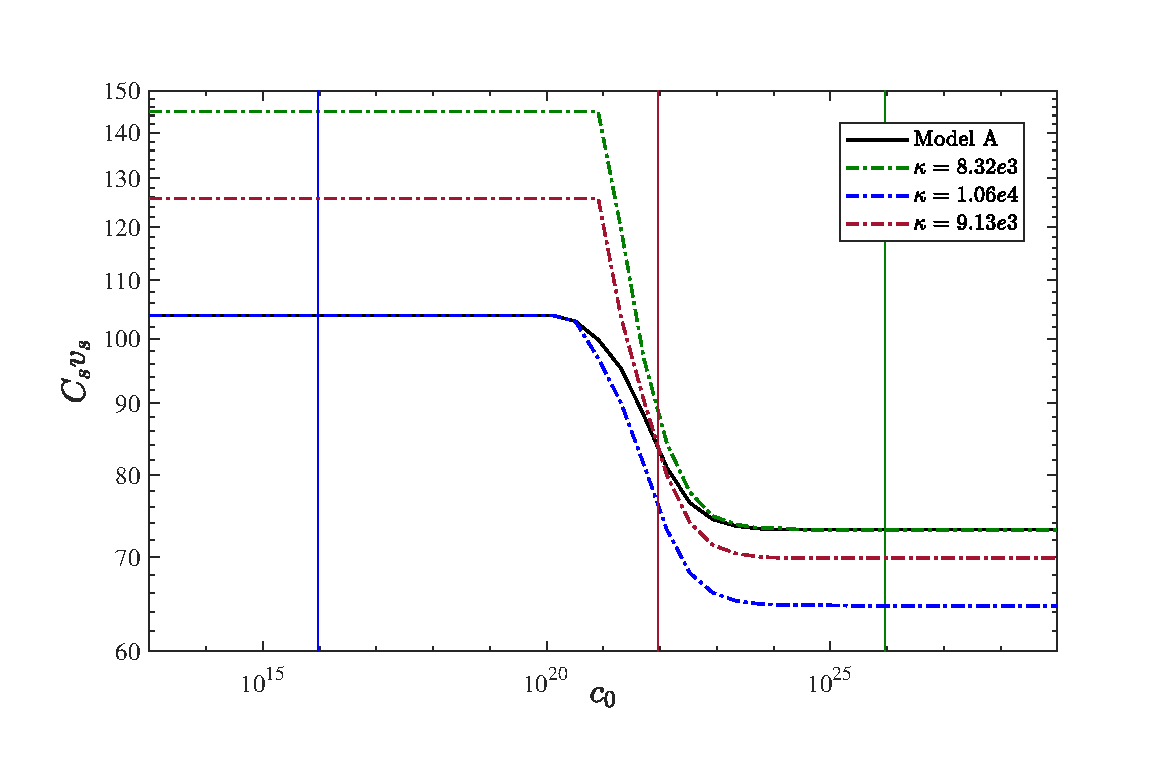
\includegraphics[scale=0.36]{images/freeswel1}
		\caption{$G^A_{eq}=5e2$}
	\end{subfigure}
	\begin{subfigure}{0.39\textwidth}
		\hspace{-8mm}
		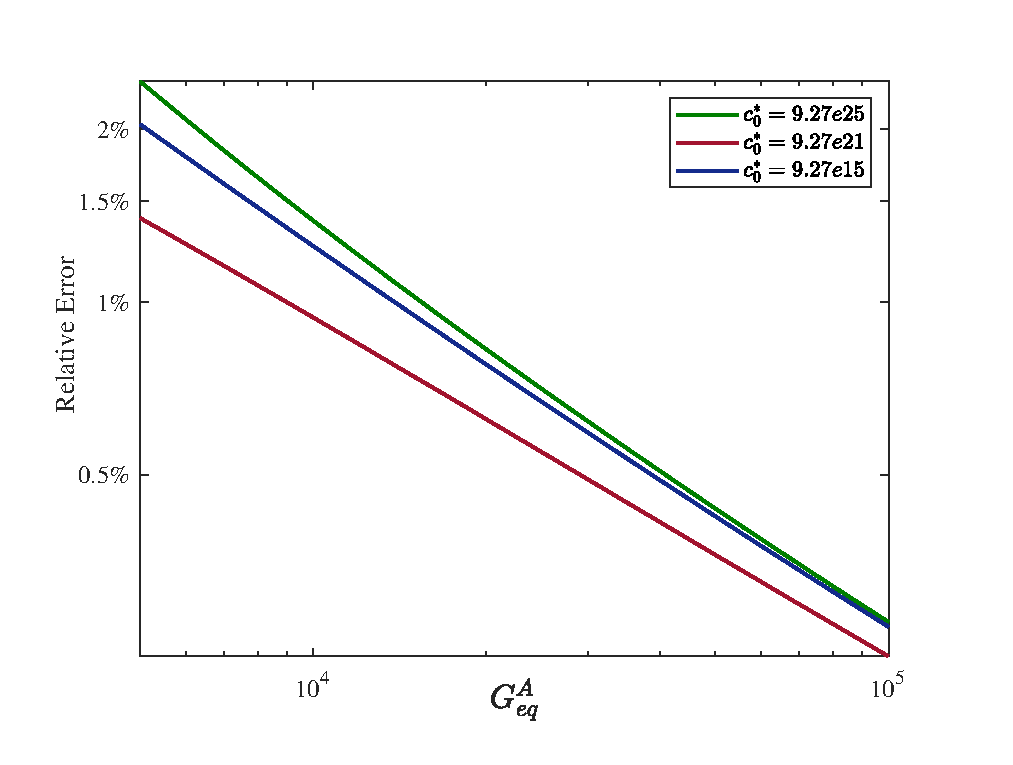
\includegraphics[scale=0.36]{images/freeswel2}
		\caption{}
	\end{subfigure}
\vspace{3mm}
\caption{Comparison of the prediction for the two models in a Free Swelling experiment. We consider as a reference Model A (ground truth). We fix the concentration $c_0=c^*_0$ of ions in the bath, we leave the matrix reach is steady state and we measure $C_s$. Given such information, we can estimate $\kappa(c^*_0)$ using Equation~(\ref{eqFb}). The experiment is repeated for a different salt concentration in the bath (each experiment correspond to a colour). (a) Using the estimated values $\kappa(c^*_0)$, we simulate an \textit{in silico} experiment and we compare it with Model A ('reality'). (b) Relative error from the \textit{in silico} experiment for the different values of $\kappa(c^*_0)$ as a function of the matrix stiffness. We note that the softer the matrix, the larger is the discrepancy between the two model. The choice of $c^*_0$ has a large impact on the error, as the model can not agree for the two limits: $c_0$ small or $c_0$ large. Note that the shear modulus of the ECM is estimated to be of order $10^3-10^4$ \cite{Netti}.}
\label{Exp1}
\end{figure}
\section{Confined Compression Test.}
<<<<<<< HEAD
In this second example, we look at another of the commonly 
=======
In this second example, we look at another of the common mechanical test used to investigate the properties of a material. This allows to measure both the dynamical and equilibrium behaviour of the material by measuring the stress while imposing a known strain $\epsilon$.
\begin{equation}
\F=J_0^{1/3}\begin{bmatrix}
1 &0&0\\
0&1&0\\
0&0& \lambda_1
\end{bmatrix}, 
\end{equation}
where $\lambda_1 = 1 - \epsilon$. 
\subsection{Model A}
As before, $\B_e$ has a structure similar to $\F$:
\begin{equation}
\B_e=\begin{bmatrix}
b &0&0\\
0&b&0\\
0&0& b_1
\end{bmatrix}. 
\end{equation}
We are first interested in the equilibrium behaviour, for which Equations~(\ref{eqion}) still holds. Focusing on the contribution of spring B, studying the equilibriums of Equation~(\ref{Be}), we obtain that $b=b_1$. Since $\det B_e= (\det F)^2$, we conclude that:
\begin{equation}
b = J_0^{2/3}\lambda_1^2.
\end{equation}

Using the boundary condition, we can now compute the pressure and the equilibrium condition:
\begin{gather}
p = -\sigma + \frac{G^A_1}{J_0\lambda_1} (J^{2/3}_0\lambda_1^2-1)+\frac{G^A_2}{J_0\lambda_1} (J_0^{2/3} \lambda_1^{2/3}-1) \\
\begin{aligned}
\frac{\sigma v_s}{k_B T}=&\frac{J_0\lambda_1+\chi}{J_0^2\lambda^2_1}+\frac{G_1^Av_s}{k_BT} \frac{J_0^{2/3}\lambda^2_1-1}{J_0 \lambda_1}+\frac{G_2^Av_s}{k_BT} \frac{J_0^{2/3}\lambda^{2/3}_1-1}{J_0 \lambda_1}\\[1.5mm]
&+\ln \frac{J_0\lambda_1-1}{J_0\lambda_1} +2c_0v_s-\sqrt{\left(\frac{z_fC_fv_s}{J_0\lambda_1-1}\right)^2+4v_s^2c^2_0}
\end{aligned}
\end{gather}
\subsection{Model B}
\begin{equation}
\bar{\B}=\begin{bmatrix}
\lambda_1^{-2/3} &0&0\\
0&\lambda_1^{-2/3}&0\\
0&0& \lambda_1^{4/3}
\end{bmatrix}, \qquad
\bar{\B}_e=\begin{bmatrix}
\bar{b} &0&0\\
0&\bar{b}&0\\
0&0& \bar{b}_1
\end{bmatrix}
\end{equation}

As for the model A, at equilibrium we have that $\bar{b}=\bar{b}_1$. However, in this case, we have that $\det \bar{B}_e=1$ so that $\bar{b}=1$ so that the second spring does not contribute to the stress. Using the boundary condition, we have that:

\begin{gather}
\displaystyle 
p = -\sigma + \frac{\kappa}{J_0\lambda_1}+\dfrac{2G^B_1}{3J_0\lambda_1^{5/3}} (\lambda_1^2-1) \\
\begin{aligned}
\frac{\sigma v_s}{k_B T}=&\dfrac{J_0\lambda_1+\chi}{J_0^2\lambda^2_1}+\frac{2G_1^Bv_s}{3k_BT} \dfrac{\lambda^2_1-1}{J_0 \lambda_1^{5/3}}+\frac{\kappa v_s}{k_BT} \frac{1}{J_0 \lambda_1}+\ln \frac{J_0\lambda_1-1}{J_0\lambda_1}\\[1.5mm]
& +2c_0v_s-\sqrt{\left(\frac{z_fC_fv_s}{J_0\lambda_1-1}\right)^2+4v_s^2c^2_0}
\end{aligned}
\end{gather}
>>>>>>> 9a98df00ba687f9a06cdcd98a853bf0b52d3dee0
%\section{Compression Test.}
%We here consider another standardd
\newpage
\appendix
\section{Glossary of Variables and Parameters in the Model.}
\begin{table}[h]
\begin{tabular}{c  l}
	$\psi\qquad $ & Helmholtz free energy per unit volume in the initial configuration,\\
<<<<<<< HEAD
	$\mathbf{u}\qquad$ & Displacement vector,\\
	$\F\qquad$ & Deformation gradient tensor $\F=\mathbb{I}-\nabla_0\mathbf{u}$,\\
=======
	$C_f\qquad$ & Concentration of fix charges in the network,\\
	$z_f\qquad$ & Charge of a GAG chain,\\
	$v_m$ & Characteristic molecular volume of the species $m$,\\
	$\mathbf{u}\qquad$ & Displacement vector,\\
	$\F\qquad$ & Deformation gradient tensor $\F=\mathbb{I}-\nabla_0\mathbf{u}$,\\	
	$\mathbb{C}\qquad$ & Right Cauchy-Green Tensor $\mathbb{C}=\F^T\F$,\\
	$\mathbb{B}\qquad$ & Left Cauchy-Green Tensor $\mathbb{B}=\F\F^T$,\\
	$\LL\qquad$ & Velocity Gradient Tensor $\LL=\dot{\F}F^{-1}$,\\
>>>>>>> 9a98df00ba687f9a06cdcd98a853bf0b52d3dee0
	$J\qquad$ & Determinant of the deformation gradient tensor $J=\det \F$,\\
	$\eta^A\qquad $ & Viscosity of the collagen network in model A,\\
	$G^A_1\qquad$ & Shear modulus related to spring $1$ in model A\\
	$G^A_2\qquad$ & Shear modulus related to spring $2$ in model A\\
	$G^B_1\qquad$ & Shear modulus related to spring $1$ in model B\\
	$G^B_2\qquad$ & Shear modulus related to spring $2$ in model B\\
	$\eta^B\qquad$ & Viscosity of the collagen network in model A,\\
	$\tau_R\qquad$ & Viscous relaxation time of the collagen network,\\
	$D_i\qquad$ & Diffusion coefficient for the $i$-th solute species when in pure solvent (interstitial fluid),\\
	$D^0_i\qquad$ & Diffusion coefficient for the $i$-th solute species in ECM,\\
	$K\qquad$ &  Hydraulic permeability of the ECM to the interstitial fluid (solvent+solute),\\
	$k\qquad$ &  Hydraulic  permeability  to  pure  solvent (water),\\
	$\kappa\qquad$ & Bulk modulus\\
	$\mathbb{T}^{Kort}\quad$ & Korteweg stress due to the ideal interface\\
	$\mathbb{T}^{Max}\quad$ & Maxwell stress due to the electric displacement\\
	$k_B\qquad$ & Boltzmann constant\\
	$\text{DEV}\left[\cdot\right]\quad$ & Deviatoric part of the tensor $\text{DEV}\left[\cdot\right] = \cdot-1/3\, \text{tr}(\cdot)$
\end{tabular}	
\end{table}
%\section{f}
%\begin{gather}
%\boldsymbol{\xi} = \frac{\partial \psi}{\partial \nabla_0 C_s},\\
%\mu_s = p v -\nabla_0 \cdot \boldsymbol{\xi} + \frac{\partial \psi}{\partial C_s},\\
%\mu_i =  e\Phi z_i +\frac{\partial \psi}{\partial C_i},\hspace{5mm} i=1,\ldots,N ,\\
%\mathbf{E} = \frac{\partial \psi}{\partial \mathbf{H}} ,\label{ele}\\
%\mathbb{S} = -p J \F^{-T} + \frac{\partial \psi}{\partial \F}+ \frac{\partial \psi}{\partial\F_e}\F_v^{-1}\, ,\\
%\zeta_m =-T^{-1} \nabla_0 \,\mu_m,\\
%\zeta_v = T^{-1} \F_e^T\frac{\partial \psi}{\partial \F_e}.
%\end{gather}
\section{Energy Dissipation.}
\label{apenergy}
Combining Equation~(\ref{vflow1}) and (\ref{vflow2}), and imposing that condition~(\ref{Jv}) is satisfied, we can characterise the viscous flow by the following relation:
\begin{equation}
\LL_v = L_{vv}T^{-1}\left[\F_e^T\frac{\partial \psi}{\partial \F_e}-p_v\mathbb{I}\right] \stackrel{(\ast)}{=} \frac{G_\mathbf{B}}{\eta^A}\text{DEV}\left[\mathbb{C}_e\right] ,
\end{equation}
where $\eta^A$ represent the viscosity of the material and the equality $(\ast)$ follows from Equation~(\ref{temp4}):
\begin{equation}
\eta^A tr(\LL_v)= tr\left(\F_e^T\frac{\partial \psi}{\partial \F_e}\right) -  3 p_v=0 \Longrightarrow  p_v = \frac{tr\left(\F_e^T\frac{\partial \psi}{\partial \F_e}\right)}{3}.
\end{equation}
Using Equation~(\ref{hyp}), we obtain:
\begin{equation}
\LL_v = \frac{G^A_2 }{\eta^A}\text{DEV}[\mathbb{C}_e] = \frac{\text{DEV}[\mathbb{C}_e]}{2\tau_R}.\label{apBe}
\end{equation}

If we now consider the left elastic Cauchy Green tensor $\mathbb{B}_e=\F_e \F^T_e$, we can relate its time derivative to $\LL_v$:
\begin{equation}
\begin{aligned}
\dot{\mathbb{B}}_e &= \LL \mathbb{B}_e + \mathbb{B}_e \LL^T - 2 \F_e d_v \F_e^{T} \\
&= \LL\mathbb{B}_e + \mathbb{B}_e \LL^T - \frac{1}{\tau_R} \F_e\left[\mathbb{C}_e-\frac{1}{3}tr(\mathbb{B}_e)\mathbb{I}\right]\F_e^T\\
&= \LL\mathbb{B}_e + \mathbb{B}_e \LL^T - \frac{1}{\tau_R} \,\mathbb{B}_e\underbrace{\left[\mathbb{B}_e-\frac{1}{3}tr(\mathbb{B}_e)\mathbb{I}\right]}_{\text{DEV}[\mathbb{B}_e]}.
\end{aligned}
\end{equation}

For what concern the dissipation due to transport phenomena, the forces $\varsigma_m$ is dependent on the deformation. For this reason, it is more suitable to move from the Lagrangian to the Eulerian coordinates.  Using the  can rewrite the flux as $\mathbf{j}_m = c_m (\mathbf{v}_m-\mathbf{v}_n)= c_m \bar{\mathbf{v}}_{m}$, where $\mathbf{v}_m$ is the velocity of the $m$-th component in the current configuration, $\mathbf{v}_n$ is the velocity of the network also in the current configuration and  $\bar{\mathbf{v}}_{m}$ is the relative velocity of the $m$-th component with respect to the network. 

In the framework of linear non-equilibrium thermodynamics, the transport dissipation function is given by:
\begin{eqnarray}
-c_j \nabla \mu_j = \sum_b L_{jb} \bar{\mathbf{v}}_j= \sum_{i\neq j} f_{ji} \left(\bar{\mathbf{v}}_i-\bar{\mathbf{v}}_j\right) + f_{js} (\bar{\mathbf{v}}_s-\bar{\mathbf{v}}_j) + f_{jn} \bar{\mathbf{v}}_j,\label{drag1}\\
-c_s \nabla \mu_s = \sum_i f_{si} \left(\bar{\mathbf{v}}_i-\bar{\mathbf{v}}_s\right)+ f_{sn} \bar{\mathbf{v}}_s,
\end{eqnarray}
where $f_{mi}$ and $h_{mn}$ are the drag coefficients related to the interaction between fluid constituents and the polymer network respectively. Based on the Onsanger's reciprocal relation we have that:
\begin{equation}
f_{mb}=f_{bm}.
\end{equation}
Common assumption in the study of mixture theory is that the solute-solute drag can be neglected so that $f_{ij}=0$ for $i,j=1,\ldots,N$ \cite{ecm1,biophysics}. The remaining drag coefficient are instead defined by:
\begin{equation}
f_{sn} = \frac{1}{k}, \ \ f_{js}=\frac{k_BT c_j}{D^0_{j}},\ \  f_{js}+f_{jn}= \frac{k_BT c_j}{D_j}, \label{drag2}
\end{equation}
where $k$ is the hydraulic permeability of the solvent in the network, $D^0_j$ is the diffusion coefficient of the solute in pure solution, while $D_j$ is the diffusion coefficient in the gel.

Using~(\ref{drag1})-(\ref{drag2}), the relative velocities are of the form:
\begin{eqnarray}
\bar{\mathbf{v}}_s = -K \left(c_s\nabla \mu_s +\sum_i \frac{D_i}{D^0_i} c_i \nabla \mu_i\right),\\
\bar{\mathbf{v}}_j = - \frac{D_j}{k_B T}\nabla \mu_j + \frac{D_j}{D^0_j} \bar{\mathbf{v}}_s, 
\end{eqnarray}
and the coefficient $K$ is defined as:
\begin{equation}
\frac{1}{K} = \frac{1}{k} + \sum_i k_B T \left(1-\frac{D_i}{D^0_i}\right) \frac{c_i}{D^0_i}.
\end{equation}

\section{Model B: Separating the Volumetric Deformation.}
The derivation of the governing equation for the second model proposed follow the same steps as model A, with few changes. From the point of view of conservation laws (Section \ref{conslaw}), these are still valid as they do not depend on the specific kinetics model chosen. As discussed in Section \ref{kin}, we use multiplicative decomposition to isolate the different contribution to the strain:
\begin{equation}
\F= \bar{\F} \F_{vol}= J^{1/3} \bar{\F}_e \bar{\F}_v,\label{mol2}
\end{equation}
where we have used the fact that $\F_{vol}=J^{1/3}\mathbb{I}$, with $J=\det \F$. Where both $\bar{\F}_e$  and $\bar{\F}_v$ needs to preserve the ECM volume. Analogously to Equation~(\ref{Jv}), this can be ensured by imposing the following condition:
\begin{equation}
\det \bar{\F}_v = 1.
\end{equation}
\begin{figure}
	\Large
	\def\svgwidth{1\linewidth}
	\input{latex/images/modelB2.pdf_tex}
	\caption{Multiplicative decomposition of Model B}
\end{figure}

In this case it is easier to express the kinematics of the ECM in terms $\LL=\dot{\F}\F^{-1}$, instead of $\dot{\F}$ and $\bar{\LL}_v=\dot{\bar{\F}}_v\bar{\F}_v^{-1}$. When we look at the free energy, we now have three decouple mechanical variables that can contribute to it $J$ for the first spring, $\bar{\F}$ and $\bar{\F}_e$ on due to the springs in branch $\mathbf{A}$ and $\mathbf{B}$ respectively. Consequently, Equation~(\ref{temp1}) will now be of the form:
\begin{equation}
\psi = \psi (J,\bar{\F}_e, \bar{\F}, C_s, C_i, \nabla_0 \,C_s,\mathbf{H}).\label{aptemp1}
\end{equation}

If we differentiate $J$, $\bar{\F}$ and $\bar{\F}_e$, we can reduce the number of variables expressing them in terms of $\LL$ and $\bar{\LL}_v$:

\begin{gather}
\dot{J} = J (\mathbb{I}:\LL),\\
\dot{\bar{\F}} = J^{-1/3} \LL \F - \frac{1}{3} J^{-1/3} (\mathbb{I}:\LL) \F \\
\dot{\bar{\F}}_e = \text{DEV}[\LL] \bar{\F}_e -\bar{\F}_e \bar{\LL}_v.\label{aptemp2}
\end{gather}
If we now combine Equations~(\ref{aptemp1})-(\ref{aptemp2}) with the energy inequality, what we obtain is:
\begin{equation}
\begin{aligned}
\left(\frac{\partial \psi}{\partial \nabla_0 C_s}-\boldsymbol{\xi}\right) \cdot \nabla_0 \dot{C}_s + \left(\frac{\partial \psi}{\partial C_s}-\mu_s-\nabla_0 \cdot \boldsymbol{\xi}+p v\right)\dot{C}_s\\
+ \sum_i\left(\frac{\partial \psi}{\partial C_i} + e\Phi z_i-\mu_i\right) \dot{C}_i +\left(\frac{\partial \psi}{\partial \mathbf{H}}-\mathbf{E}\right) \cdot \dot{\mathbf{H}}\\
 +\left(\text{DEV}\left[J^{-1/3}\frac{\partial \psi}{\partial \bar{\F}}\F^T + \frac{\partial \psi}{\partial \bar{\F}_e}\bar{\F}_e^{T}\right]- \mathbb{S}\F^T +J\left(\frac{\partial \psi}{\partial J} - p\right)\mathbb{I}\right):\LL\\
 + \sum_m \nabla_0 \,\mu_m \cdot \mathbf{J}_m - \bar{\F}_e^T\frac{\partial \psi}{\partial \bar{\F}_e}:\mathbb{\bar{L}}_v\leq 0 . \label{ineq2}
\end{aligned}
\end{equation}

Finally we need to update the constitutive laws for the strain free energy $\psi_6$, which, similarly to the case discussed in Section , can be decompose as the sum of contributions from each spring in Figure \ref{figmode}(b):

\begin{equation}
\psi_6 = \psi_1(\bar{\F}) + \psi_2(\bar{\F}_e) + \psi_{vol}(J).
\end{equation}

Again we assume the ECM to behave as an hyperplastic material:
\begin{eqnarray}
\psi_1(\bar{\F}) = \frac{G^B_1}{2} \left(\bar{\F}:\bar{\F} - 3\right),\\
\psi_2(\bar{\F}_e) = \frac{G^B_2}{2} \left(\bar{\F}_e:\bar{\F}_e - 3 \right).
\end{eqnarray}

For the volumetric contribution we consider as before a logarithmic term:
\begin{equation}
\psi_{vol}(J) = \frac{\kappa}{2} \ln J^2.
\end{equation}

The above volumetric constitutive assumption is one of the most common in modelling hyper-elastic material. However, as shown in \cite{vol}, this has several limitation in the regime of large deformation, which highlights the need of study more realistic form which can capture the more complex behaviour of real material. From this point of view, being able to decouple the volumetric deformation as in model B allows to investigate this aspect alone [REPHRASE].

When looking at the entropy production, Equation~(\ref{dis}) still holds simply by replacing $\LL_v$ with $\bar{\LL}_v$. Using the same argument as in Section~(\ref{ent}), we are left with the following system of equations:
\begin{gather}
\boldsymbol{\xi} = \gamma J \,\mathbb{B}^{-1} \,\nabla_0 \,C_s,\label{sys1B}\\[2mm]
\begin{aligned}
\mu_s = p v + \mu_s^0 - \gamma J \nabla^2 C_s + kT&\left[\ln \frac{C_s v}{1+C_s v} + \frac{1}{1+C_sv}\right.\\
&\left.\ \ \ \ \ \ +\frac{\chi}{(1+C_s v)^2}-\sum_i \frac{C_i}{C_s}\right], 
\end{aligned}\\[2.5mm]
\mu_i = \mu^0_i + e\Phi z_i + kT \ln \frac{C_i}{C_s},\\
\mathbf{E} = \frac{1}{\epsilon J} \F^T \F\, \mathbf{H}\, \\[3mm]
\begin{aligned}
\mathbb{T}= \left(\frac{\kappa}{1+C_sv_s}-p\right) \mathbb{I} + \frac{G^B_1}{1+C_sv}\text{DEV}[\bar{\B}] + \frac{G^B_2}{1+C_sv}\text{DEV}[\bar{\B}_e]\\
+ \gamma \left[\frac{1}{2} |\nabla C_s|^2\mathbb{I} - \nabla C_s \otimes \nabla C_s\right]+ \epsilon \left[\frac{1}{2} \,|\nabla \Phi|^2\mathbb{I} -\nabla \Phi \otimes \nabla \Phi\right],\label{sys2B}
\end{aligned}
\end{gather}
coupled to the governing equations:
\begin{gather}
\mathbf{j}_s = -K c_s \left(c_s\nabla \mu_s +\sum_i \frac{D_i}{D^0_i} c_i \nabla \mu_i\right),\\
\mathbf{j}_i = - \frac{D_i}{k_B T}c_i\nabla \mu_i + \frac{D_i}{D^0_i} \frac{c_i}{c_s} \mathbf{j}_s, \\
\dot{\bar{\B}}_e = \bar{\B}_e \LL^T +\LL \bar{\B}_e - \frac{2}{3} \, tr(\LL) \bar{\B}_e -\frac{1}{\tau_R} \bar{\B}_e \text{DEV}\left[\bar{\B}_e\right]
\end{gather}
%\section{Korteweg stress terms.}
The Korteweg stress is the part of the mechanical stress which is related to the interfacial free energy. We here report the result related to the second model. This will have a contribution from the both the derivative with respect to $\bar{F}$ and $J$:
\begin{equation}
\mathbb{T}^{korg} = \text{DEV}\left[J^{-1}\frac{\partial \psi_{int}}{\partial \bar{\F}}\bar{\F}^T\right] + \frac{\partial \psi_{int}}{\partial J} \mathbb{I}
\end{equation}
where the interface energy is given by:
\begin{equation}
\psi_{int}(J,\bar{F}) = \frac{\gamma}{2} J^{1/3} \bar{\F}^{-1}\bar{\F}^{-T} \left|\nabla_0 C\right|^2.
\end{equation}
Using the properties of the deformation tensor $\bar{F}$, it can be shown that:
\begin{equation}
\frac{\partial }{\partial \bar{\F}} \left(\bar{\F}^{-1} \bar{\F}^{-T} \left|\nabla_0 C\right|^2\right) \bar{\F}^T = -2 J^{2/3} \,\nabla C \otimes \nabla C,
\end{equation} 
so that the Korteweg stress is given by:
\begin{equation}
\mathbb{T}^{korg} = - \gamma \text{DEV} \left[ \nabla C \otimes \nabla C\right] + \frac{\gamma}{6} \left|\nabla C\right|^2 \mathbb{I}.
\label{kor}
\end{equation}
If we now explicitly evaluate the deviatoric component we have:
\begin{equation*}
\begin{aligned}
tr(\nabla C \otimes \nabla C) = \left|\nabla C\right|^2 \\ \text{DEV}\left[\nabla C \otimes \nabla C\right] = \nabla C \otimes \nabla C -\frac{\left|\nabla C\right|^2}{3} \mathbb{I}.
\end{aligned}
\end{equation*}
Substituting now the expressions back in Equation~(\ref{kor}), we obtain:
\begin{equation}
\mathbb{T}^{korg} = \gamma \left[\frac{1}{2} \left|\nabla C\right|^2 \mathbb{I} - \nabla C \otimes \nabla C\right],
\end{equation}
which is equivalent to result obtained for the first model.

%The dissipative contribution due to the relative movement of phases has been largely studied in the literature \cite{ecm1,ecm2}. Starting from Equation~(\ref{dif}) and standard arguments we can get to the following definition for the fluxes:\
\newpage
\bibliographystyle{splncs04}
\bibliography{latex/ref}
%
\end{document}
